% !TEX TS-program = pdflatex

\documentclass[unicode,11pt,notheorems]{beamer}

\usepackage[T2A]{fontenc}
\usepackage[utf8]{inputenc}
\usepackage[russian]{babel}
\usepackage{amsmath,amsfonts,amssymb,amsthm}
\usepackage{mathtools}

\usepackage{xcolor,colortbl,tabularx,array}
\usepackage{ulem}
\usepackage{tikz, graphicx}
%\usepackage{tkz-graph}
\usetikzlibrary{matrix,arrows,decorations.pathmorphing, arrows.meta,positioning}
\usetikzlibrary{positioning,calc}
\usetikzlibrary{petri}
\usetikzlibrary{decorations.pathreplacing}

%Описание стиля презентации
\usetheme[sidebar=0]{kfmn} 
\setbeamercovered{transparent}

%\definecolor{cyan}{RGB}{240,217,1}
%\definecolor{vgugreen}{RGB}{143,188,103}
%\definecolor{vgured}{RGB}{234,38,40}
%\definecolor{vgublue}{RGB}{53,101,167}

\newcommand{\myunit}{9mm}
\tikzset{
    node style sp/.style={draw,circle,minimum size=\myunit},
    node style ge/.style={circle,minimum size=\myunit},
    arrow style mul/.style={draw,sloped,midway,fill=white},
    arrow style plus/.style={midway,sloped,fill=white},
}

%[0, 6, 8, 8, 10, 5, 6, 10, 8, 10, 10], 

\pgfdeclareimage[height=8mm]{university-logo}{logo-iem.png}
\logo{\pgfuseimage{university-logo}}
%2[0, 11, 10, 8, 11, 5, 11, 11, 8, 11, 10, 11],

\titlepicture{
	\begin{tikzpicture}[y=1.4cm,overlay,rotate=8]
	\coordinate (O) at (-3cm,0.9cm);
	\filldraw[thick,draw= vgublue, fill=vgublue!20!white] (0,0) circle[radius=4.2cm];
	\clip (0,0) circle[radius=4.2cm];
	\draw (-1.5,1.5) node{
	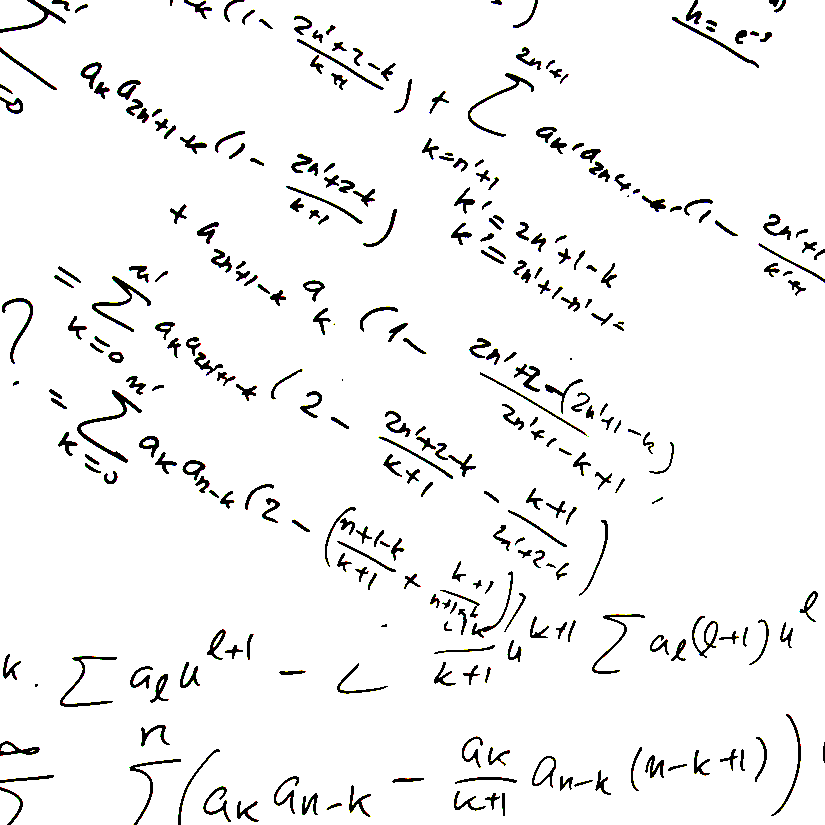
\includegraphics[width=8cm]{titlepic.png}
	};
\end{tikzpicture}
}

\usepackage[math]{iwona}

\newcommand{\hplus}{\mathbin{\hat+}}
\newcommand{\hdot}{\mathbin{\hat\cdot}}
% Описание теорем
\newtheorem{theorem}{Теорема}
\newtheorem{seq}{Следствие}
%%

%\VKR
\LECT % можно ещё лекцию забацать.
%\REPORT % можно ещё лекцию забацать.

%\titlepicture{
%%	\begin{tikzpicture}[overlay]
%%			\draw[opacity=0.4]  (-0.3,1.8) node {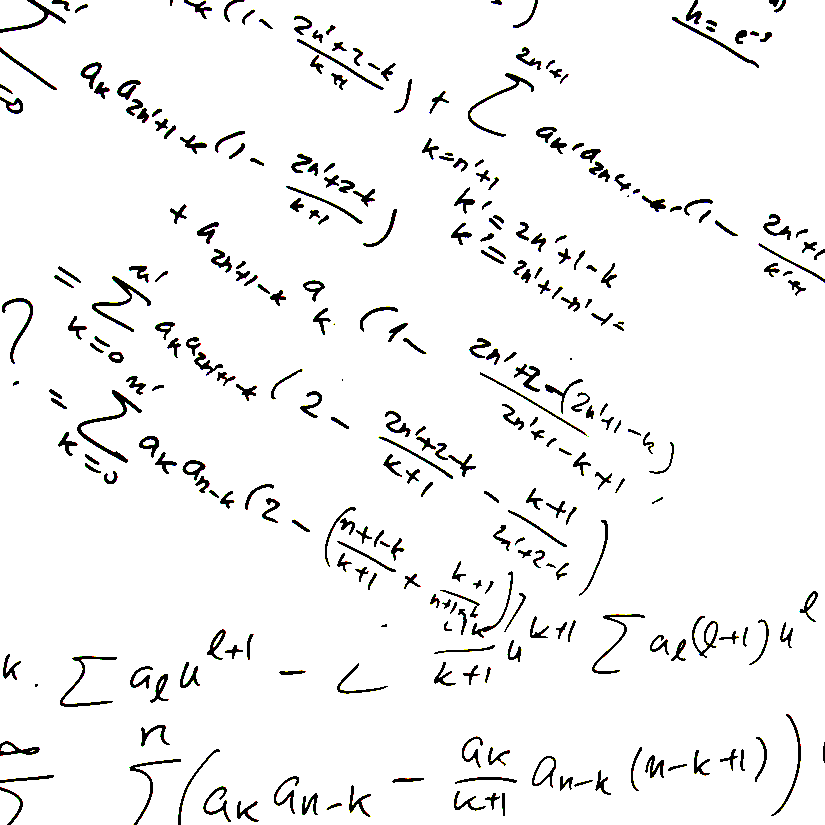
\includegraphics[width=3.5cm]{titlepic.png}};
%%	\end{tikzpicture}
%}

% Титульный лист теорем
\author[Д.\,В. Чупраков]{канд.\,физ.-матем.\,наук, доцент Д.\,В. Чупраков\\[6pt] usr10381@vyatsu.ru}

\institute[ВятГУ]{ФГБОУ ВО Вятский государственный университет}

\department{Факультет экономики и финансов}

\title[Лекция~5. Линейные задачи. Часть~3 из 4]{
	Введение в экономико-математическое моделирование\\[12pt]
	Лекция 5. Линейные задачи--3}
\subtitle{Задача линейного программирования. Методы ее решения. Устойчивость}


\date{05 октября 2020 г.}


%\setbeamercolor{coloredboxstuff}{fg=yellow,bg=white!10!blue}

\setbeamercovered{invisible}


\tikzset{
	 myarrow/.style={->, >=latex', shorten >=1pt, thick}
}



\tikzset{add/.style n args={4}{
    minimum width=6mm,
    path picture={
        \draw[black] 
            (path picture bounding box.south east) -- (path picture bounding box.north west)
            (path picture bounding box.south west) -- (path picture bounding box.north east);
        \node at ($(path picture bounding box.south)+(0,0.13)$)     {\tiny #1};
        \node at ($(path picture bounding box.west)+(0.13,0)$)      {\tiny #2};
        \node at ($(path picture bounding box.north)+(0,-0.13)$)        {\tiny #3};
        \node at ($(path picture bounding box.east)+(-0.13,0)$)     {\tiny #4};
        }
    }
}

\tikzset{bigadd/.style n args={4}{
    minimum width=20mm,
    path picture={
        \draw[black] 
            (path picture bounding box.south east) -- (path picture bounding box.north west)
            (path picture bounding box.south west) -- (path picture bounding box.north east);
        \node at ($(path picture bounding box.south)+(0,0.5)$)     { #1};
        \node at ($(path picture bounding box.west)+(0.5,0)$)      {#2};
        \node at ($(path picture bounding box.north)+(0,-0.5)$)        {#3};
        \node at ($(path picture bounding box.east)+(-0.5,0)$)     {#4};
        }
    }
}



\usepackage{mathtools}
\usepackage{pifont}
\newcommand{\verteq}{\rotatebox{90}{$\,=$}}
\newcommand{\equalto}[2]{\underset{\scriptstyle\overset{\mkern4mu\verteq}{#2}}{#1}}

\begin{document}


\maketitle

\begin{frame}{Структура лекции}
	\tableofcontents
\end{frame}


%\section{Экономические задачи, приводящие к понятию матриц}


%\section{Графический метод решения ЗЛП}
\section{Геометрический смысл системы ограничений ЗЛП}

\begin{frame}[t]{}{}
\vspace{2cm}
{\LARGE Геометрический смысл\\ системы ограничений\\ задачи линейного программирования\par}
\vspace{\fill}

\end{frame}   

\subsection{Выпуклые множества}

\begin{frame}{Выпуклые множества}{}
\begin{tabular}{m{0.65\textwidth}m{0.33\textwidth}}
\structure{Определение}

Множество $\Phi$ \alert{выпуклое} если 
 
{\centering $A,B \in \Phi \Rightarrow AB\subseteq \Phi $\par} &
\begin{tikzpicture}[x=0.5cm,y=0.5cm]
	\filldraw[draw=black,fill=green!20] (0,0)-- (1,2)-- (3,1) -- (2,-2) -- (1,-1) --cycle;
	\filldraw[draw=black,fill=black] (1,1) circle[radius=1pt] node[above] {$A$} -- (2,0) circle[radius=1pt] node[above] {$B$};
\end{tikzpicture}
\begin{tikzpicture}[x=0.5cm,y=0.5cm]
	\filldraw[draw=black,fill=red!20] (0,1)-- (2,1.5) -- (1,-1) -- (3,1) -- (2,-2) -- (0.5,-1) --cycle;
	\filldraw[draw=black,fill=black] (0.5,0.5) circle[radius=1pt] node[above] {$A$} -- (2,-1) circle[radius=1pt] node[above] {$B$};
\end{tikzpicture}
\end{tabular}

\structure{Свойства}

\begin{itemize}
	\item $\Phi$~--- выпуклое $\Leftrightarrow$ $C=\alpha A+\beta B \in \Phi$ для любых $A,B \in \Phi$, $\alpha+\beta=1$.  
	\item 
		\alert{$a_{1} x_1 + a_{2} x_2 + \ldots + a_{n} x_n= b$}~--- выпуклое множество
	\item 
		Пересечение выпуклых множеств~--- выпуклое множество
\end{itemize}

\begin{theorem}
	Множество всех планов задачи линейного программирования выпукло.
\end{theorem}

\end{frame}


\begin{frame}{Теорема об оптимальном значении}{}
\begin{theorem}
	Целевая функция задачи линейного программирования достигает своего оптимального значения в угловой вершине многоугольника решений. 
\end{theorem}

%\pause
%\structure{Идея:} 
%$$
%	A \in \Phi
%$$
%	$$
%		A=\alpha_1 A_1 + \alpha_2 A_2
%	$$
%	$$
%	\alpha_1 + \alpha_2 =1, \quad A_1,A_2 \text{ --- граничные точки}
%	$$
%	$$
%		F(A)=?
%	$$
%
%\visible<2->{
%	\structure{Доказательство}
%	
%	Пусть $A(x_1,\ldots x_n)$ не угловая и $F(A)$~--- наибольшее значение.
%
%	Найдём граничную точку~$B$, что $F(A)=F(B)$.
%
%	{\centering
%		$A=\alpha_1 A_1 + \alpha_2 A_2$,\\
%		$\alpha_1 + \alpha_2 =1, \quad A_1,A_2 \text{ --- граничные точки}$\\[1em]
%		${\color<2>{red} F(A)}=\alpha_1 F(A_1)+ \alpha_2 F(A_2) 
%		\visible<2->{{\color<2>{red}\leqslant} \alpha_1 B+ \alpha_2 B = (\alpha_1 +\alpha_2)F(B) = {\color<2>{red}F(B)}}$\\
%		\only<3>{
%			\color{red}
%				$F(B) \leqslant F(A) \leqslant F(B)$\\
%		}
%		\only<4->{
%			\color<4>{red}
%				$F(A) = F(B)$\\
%		}\par
%	}
%	\only<5->{Итак, целевая функция принимает наибольшее значение в~граничной точке~$B$.
%	
%	Аналогично,	$B=\alpha_1 B_1 + \alpha_2 B_2$, где $B_1$,$B_2$~--- угловые.
%	}
%}
\end{frame}   
%
%
%


\section{Графический метод решения ЗЛП}
\begin{frame}[t]{}{}
\vspace{2cm}
{\LARGE	Графический метод решения\\ задачи линейного программирования\par}
\vspace{\fill}

{\begin{alertblock}{Графический метод}
применяется для решения задач линейного программирования, зависящих от двух переменных
\end{alertblock}}
\end{frame}   

\subsection{Обоснование графического метода}
\begin{frame}{Обоснование графического метода}{}
   Графический метод основан на геометрической интерпретации задачи линейного программирования
   \begin{itemize}
		\item \structure{$F=c_1x_1+c_2x_2$}~--- уравнение прямой при каждом~$F$
		\item Ограничение \structure{$a_{k1} x_1 + a_{k2}x_2   \leqslant b_k$}~--- уравнение полуплоскости
		\item \structure{Система ограничений} --- выпуклая многоугольная область
		  \structure{
		  $$
		  \left\lbrace
		  \begin{aligned}
			  a_{11} x + a_{12}y  &\leqslant b_1\\
			  a_{21} x + a_{22}y &\leqslant b_2\\
			  &\ldots\\
			  a_{m1} x + a_{m2}y &\leqslant b_m
		  \end{aligned}
		  \right. \quad
		  \begin{aligned}
				x &\geqslant 0 \\
				y &\geqslant 0 \\
		 \end{aligned}
		  $$
		  }
   \end{itemize}
\end{frame} 

\begin{frame}{Обоснование графического метода}{}
\begin{theorem}
Значения функции $F=c_1 x+c_2 y$ возрастают в~направлении вектора~$\vec{n}=(c_1,c_2)$.
\end{theorem}
\visible<2->{
	\structure{Доказательство}\par
	\begin{itemize}
	\item<2-> $l\colon F=c_1 x_1+c_2 x_2$, \qquad $\vec{n}=(c_1,c_2) \color<2>{red}\perp l$

	\item<2-> Сдвиг~$l$ на вектор \structure{$k\vec{n}$}: 
	$$\left\lbrace\begin{aligned} x'=x+kc_1,\\ y'=y+kc_2, \end{aligned}\right. \quad k>0$$ 

	\item<2->[] $
		F'= \only<2>{c_1 x'+c_2 y' =}  
			\only<3->{c_1(x+kc_1)+c_2(y+kc_2) =} 
			\only<3->{\underbrace{c_1 x+c_2 y}_{\color{red}=F} +\underbrace{k(c_1^2+c_2^2)}_{\color{red}>0} \color{red} > F}
	$
	\end{itemize}
}
\end{frame} 

\subsection{Алгоритм графического метода}
\begin{frame}<1>[label=frm:algorithm]{Алгоритм графического метода}
\begin{enumerate}
	\item Построить область ограничений
	\item Построить опорную прямую $l\colon F=c_1x+c_2y$ при $F=0$
	\item Построить вектор $\vec{n}=(c_1,c_2)$
	\item Прямую~$l$ в область ограничений!
	\item Двигать~$l$, пока она не выйдет из области ограничений
	\begin{itemize}
		\item \alert{для $\max$:} по вектору $\vec{n}$
		\item \alert{для $\min$:} против вектора $\vec{n}$
	\end{itemize}
	\item Найти координаты последней угловой точки~$P$ пересечения прямой с областью ограничений
	\item Найти значение $F$ в~точке~$P$
\end{enumerate}
\end{frame} 
   
\subsection{Пример применения графического метода}
  
\begin{frame}{Построение области ограничений}{}
\begin{minipage}{0.47\textwidth}
 $\left\lbrace
  \begin{aligned}
    \color{red} x+3y & \color{red}\leqslant 21\\
    \color{green!50!black} 3x+2y & \color{green!50!black} \leqslant 21\\
    \color{blue}  x &\color{blue}\leqslant 5\\
    \color{orange} 3x+5y &\color{orange}\geqslant 15
  \end{aligned}
  \right.\quad
  \begin{aligned}
    x \geqslant 0\\
    y \geqslant 0
  \end{aligned}   
  $
\begin{enumerate}
\item Построение $\color{red} x+3y  \leqslant 21$
\visible<6->{
\item Построение $\color{green!50!black} 3x+2y \leqslant 21$
\item Построение $\color{blue} x \leqslant 5$
}
	\visible<2-5>{
	\begin{itemize}
		\item Построение границы: $\color{red} x+3y  = 21$\par
			\begin{tabular}{c|c|c}
				$x$ & {0} & {6}\\
				\hline
			 	$y$ & {7} & {5}
			\end{tabular}
		\visible<4->{
		\item Выбор полуплоскости: $C(1,2) \notin AB$
		
		$ 1+3\cdot 2=7  \;{\color{red}\leqslant}\; 21$
		
		}
	\end{itemize}
	} 
\end{enumerate}

\end{minipage}
\begin{minipage}{0.5\textwidth}
\begin{tikzpicture}[x=6mm,y=6mm,
			declare function={
				fua(\x)=(-\x/3+7);
				fub(\x)=(-(3/2)*\x+(21/2));
				fuc(\x)=(-(3/5)*\x+3);
			},
	 shtrih/.style={
        postaction={draw,decorate,decoration={border,angle=-45,
                    amplitude=1mm,segment length=1.5mm}}}			
			]
	\clip (-1,-1) rectangle (9,9);
	\path[name path=L1] (-1,{fua(-1)})--(9,{fua(9)});
	\path[name path=L2] (-1,{fub(-1)})--(9,{fub(9)});
	\path[name path=L3]  (5,9)--(5,-1);
	\path[name intersections={of=L1 and L2}] (intersection-1) coordinate (E);
	\path[name intersections={of=L2 and L3}] (intersection-1) coordinate (F);
	\fill<7->[fill=cyan!20] (0,0)--(0,{fua(0)}) -- (E) -- (F) --(5,0) -- (0,{fuc(0)}) --cycle;
	\draw[->] (-1,0)--(9,0) node[below left] {$x$};
	\draw[->] (0,-1)--(0,9) node[below left] {$y$};
	\draw (0,0) node[below left] {$0$};
	\draw<2>[thin, dashed, draw=red] 
		(0,7) node[left]{$7$}
		(0,5) node[left]{$5$} -- (6,5) -- (6,0) node[below]{$6$};
	\fill<2-5>[thick, fill=red] 
		(0,7) circle[radius=1.5pt] node[above right, text=red]{$A$}
		(6,5) circle[radius=1.5pt]node[above right, text=red]{$B$};
		
	\draw<4-5>[thin, dashed, draw=red] 
		(0,2) node[left]{$2$} -- (1,2) -- (1,0) node[below]{$1$};

	\fill<4-5>[thick, fill=red] 
		(1,2) circle[radius=1.5pt] node[above right, text=red]{$C$};
	\draw<3-4>[thick, color=red] (-1,{fua(-1)})--(9,{fua(9)});
	\draw<5->[thick, color=red, shtrih] (-1,{fua(-1)})--(9,{fua(9)});
	\draw<6->[thick, color=green!50!black,shtrih] (-1,{fub(-1)})--(9,{fub(9)});
	\draw<6->[thick, color=orange,shtrih] (9,{fuc(9)})--(-1,{fuc(-1)});
	\draw<6->[thick, color=blue,shtrih] (5,9)--(5,-1);
\end{tikzpicture}
\end{minipage}
\end{frame} 





\begin{frame}{Решение задачи линейного программирования}{}
\begin{minipage}{0.47\textwidth}
 $\left\lbrace
  \begin{aligned}
    \color{red} x+3y & \color{red}\leqslant 21\\
    \color{green!50!black} 3x+2y & \color{green!50!black} \leqslant 21\\
    \color{blue}  x &\color{blue}\leqslant 5\\
    \color{orange} 3x+5y &\color{orange}\geqslant 15
  \end{aligned}  \right.\quad
  \begin{aligned}
    x \geqslant 0\\
    y \geqslant 0
  \end{aligned}   
 $
 
 \medskip
$F=x+2y \to max$
\medskip
\hrule
\smallskip
\visible<2->{
\begin{itemize}
	\item $F=0$\quad $x+2y=0$
	\item<3-> $\vec{n}=(1,2)$
	\item<4-> Перемещение прямой
	\item<10->  $ P_{\max}\colon\!\left\lbrace
				  \begin{aligned}
			    \color{red} x+3y & \color{red}=21\\
				    \color{green!50!black} 3x+2y & \color{green!50!black} = 21\\
				  \end{aligned}\right.
				$
	\item<11->$P_{\max}(3,6)$
	\item<12-> $F_{\max}=F(3,6)=15$
\end{itemize}
}
\end{minipage}
\begin{minipage}{0.5\textwidth}
\begin{tikzpicture}[x=6mm,y=6mm,>=latex,
			declare function={
				fua(\x)=(-\x/3+7);
				fub(\x)=(-(3/2)*\x+(21/2));
				fuf(\x,\f)=(\f-\x)/2;
				fuc(\x)=(-(3/5)*\x+3);
				},
	 shtrih/.style={
        postaction={draw,decorate,decoration={border,angle=-45,
                    amplitude=1mm,segment length=1.5mm}}}			
			]
	\clip (-1,-1) rectangle (9,9);
	\path[name path=L1] (-1,{fua(-1)})--(9,{fua(9)});
	\path[name path=L2] (-1,{fub(-1)})--(9,{fub(9)});
	\path[name path=L3]  (5,9)--(5,-1);
	\path[name intersections={of=L1 and L2}] (intersection-1) coordinate (E);
	\path[name intersections={of=L2 and L3}] (intersection-1) coordinate (F);
	\fill[fill=cyan!20] (0,0)--(0,{fua(0)}) -- (E) -- (F) --(5,0) -- (0,{fuc(0)}) --cycle;	
	\draw[->] (-1,0)--(9,0) node[below left] {$x$};
	\draw[->] (0,-1)--(0,9) node[below left] {$y$};
	\draw (0,0) node[below left] {$0$};
	\draw[color=red, shtrih] (-1,{fua(-1)})--(9,{fua(9)});
	\draw[color=green!50!black,shtrih] (-1,{fub(-1)})--(9,{fub(9)});
	\draw[color=blue,shtrih] (5,9)--(5,-1);
	\draw[color=orange,shtrih] (9,{fuc(9)})--(-1,{fuc(-1)});	
	\draw<2->[thick,draw=black!40] (-1,{fuf(-1,0)})
					-- node[sloped,pos=0.25,above=-0.5mm]{\small $F=0$} 
				(9,{fuf(9,0)});
	\draw<3->[thick,draw=cyan,->] (0,{fuf(0,0)})
				-- node[sloped,above=-0.5mm,text=cyan]{\small $\vec{n}=(1,2)$} 
			+(1,2);

	\draw<4->[thick,draw=black!50,fill=black!50] (-1,{fuf(-1,5)}) 
	 -- node[sloped, pos=0.35, below=-0.5mm]{\small $F=F_{\min}$}
	(9,{fuf(9,5)})
									 	 (5,0) circle[radius=1.5pt] 
									 	 node[above right]{$P_{\min}$};	

	\draw<5>[thick,draw=black!60,fill=black!60] (-1,{fuf(-1,6)}) -- (9,{fuf(9,6)})
									 	 (0,{fuc(0)}) circle[radius=1.5pt] 
									 	 node[above right]{$P_1$};	

	\draw<6>[thick,draw=black!60,fill=black!60] (-1,{fuf(-1,11)}) -- (9,{fuf(9,11)})
									 	 (F) circle[radius=1.5pt] 
									 	 node[above right]{$P_2$};	
	\draw<7>[thick,draw=black!70,fill=black!70] (-1,{fuf(-1,14)}) -- (9,{fuf(9,14)})
									 	 (0,{fua(0)}) circle[radius=1.5pt] 
									 	 node[above right]{$P_3$};		
	\draw<8,10->[thick,draw=black,fill=black] 
							(-1,{fuf(-1,15)}) 
								-- node[sloped, pos=0.9, below=-0.5mm]{\small$F=F_{\max}$} 
							(9, {fuf(9,15)}) 
							(E) circle[radius=1.5pt]  
							 	 node[above right]{$P_{\max}$};		
	\draw<9>[thick,black!30,fill=black!30] (-1,{fuf(-1,16)}) -- (9,{fuf(9,16)});		
	\draw<11->[thin, dashed, draw=black] 
		(0,6) node[left]{$6$} -- (E) -- (3,0) node[below]{$3$};		
\end{tikzpicture}
\end{minipage}
\end{frame} 


\begin{frame}{Решение задачи линейного программирования}{}
\begin{itemize}
\item\structure{Математическая модель:}
	\begin{itemize}
	\item Система ограничений:\par
	\alert{\centering 
	 $\left\lbrace
	  \begin{aligned}
	    x+3y &  \leqslant 21\\
	    3x+2y &  \leqslant 21\\
	    x & \leqslant 5\\
	    3x+5y & \geqslant 15
	  \end{aligned}  \right.\quad
	  \begin{aligned}
	    x \geqslant 0\\
	    y \geqslant 0
	  \end{aligned}   
	 $\par}
	\item Целевая функция\par
		\alert{\centering $F=x+2y \to max$\par}
	\end{itemize}
	\bigskip
	\item \structure{Результат исследования модели:}
	\begin{itemize}
		\item Оптимальный план: \par
			\alert{\centering $x=3, y=6$\par}
		\item Целевая функция достигает оптимального значения: \par
		\alert{\centering $F_{\max}= 15$\par}
	\end{itemize}
\end{itemize}

\end{frame} 

%\againframe{frm:algorithm}

\subsection{Виды областей ограничений}

\begin{frame}{Ограниченная область}
\begin{minipage}{0.47\textwidth}
	Любая целевая функция имеет минимальный и максимальный планы
\end{minipage}
\begin{minipage}{0.50\textwidth}
	\begin{tikzpicture}[x=6mm,y=6mm,
				declare function={
					fua(\x)=(\x/3+5);
					fub(\x)=(-(3/2)*\x+(21/2));
				},
		 shtrih/.style={
	        postaction={draw,decorate,decoration={border,angle=-45,
	                    amplitude=1mm,segment length=1.5mm}}}			
				]
		\clip (-1,-1) rectangle (9,9);
		\path[name path=L1] (-1,{fua(-1)})--(9,{fua(9)});
		\path[name path=L2] (-1,{fub(-1)})--(9,{fub(9)});
		\path[name path=L3]  (5,9)--(5,-1);
		\path[name intersections={of=L1 and L2}] (intersection-1) coordinate (E);
		\path[name intersections={of=L2 and L3}] (intersection-1) coordinate (F);
		\fill[fill=green!20!white] (0,0)--(0,{fua(0)}) -- (E) -- (F) --(5,0) --cycle;
		\draw[->] (-1,0)--(9,0) node[below left] {$x_1$};
		\draw[->] (0,-1)--(0,9) node[below left] {$x_2$};
		\draw (0,0) node[below left] {$0$};
		\draw[color=green!50!black, shtrih] (-1,{fua(-1)})--(9,{fua(9)});
		\draw[color=green!50!black,shtrih] (-1,{fub(-1)})--(9,{fub(9)});
		\draw[ color=green!50!black,shtrih] (5,9)--(5,-1);
	\end{tikzpicture}
\end{minipage}
\end{frame} 

\begin{frame}{Неограниченная область}
\begin{minipage}{0.47\textwidth}
Возможен \alert{неограниченный оптимум}~---
	ситуация, когда для любого допустимого плана существует другой допустимый 
	план, которому соответствует лучшее значение целевой функции
\bigskip

\structure{На практике:}\\
скорее всего, при построении модели пропущено ограничение

\end{minipage}
\begin{minipage}{0.50\textwidth}
	\begin{tikzpicture}[x=6mm,y=6mm,
				declare function={
					fua(\x)=(\x/2+3);
					fub(\x)=(-(1/4)*\x+4);
				},
		 shtrih/.style={
	        postaction={draw,decorate,decoration={border,angle=-45,
	                    amplitude=1mm,segment length=1.5mm}}}			
				]
		\clip (-1,-1) rectangle (9,9);
		\path[name path=L1] (-1,{fua(-1)})--(9,{fua(9)});
		\path[name path=L2] (-1,{fub(-1)})--(9,{fub(9)});
		\path[name intersections={of=L1 and L2}] (intersection-1) coordinate (E);
		\fill[fill=yellow!20] (E)--(9,{fua(9)}) -- (9,{fub(9)})--cycle;
		\draw[->] (-1,0)--(9,0) node[below left] {$x_1$};
		\draw[->] (0,-1)--(0,9) node[below left] {$x_2$};
		\draw (0,0) node[below left] {$0$};
		\draw[color=red!70!black, shtrih] (-1,{fua(-1)})--(9,{fua(9)});
		\draw[color=red!70!black,shtrih] (9,{fub(9)})--(-1,{fub(-1)});
	\end{tikzpicture}
\end{minipage}
\end{frame}

\begin{frame}{Вырожденная область}
\begin{minipage}{0.47\textwidth}
		Минимальный и максимальные планы совпадают
\end{minipage}
\begin{minipage}{0.50\textwidth}
	\begin{tikzpicture}[x=6mm,y=6mm,
				declare function={
					fua(\x)=(-\x/3+7);
					fub(\x)=(-(3/2)*\x+(21/2));
				},
		 shtrih/.style={
	        postaction={draw,decorate,decoration={border,angle=-45,
	                    amplitude=1mm,segment length=1.5mm}}}			
				]
		\clip (-1,-1) rectangle (9,9);
		\path[name path=L1] (-1,{fua(-1)})--(9,{fua(9)});
		\path[name path=L2] (-1,{fub(-1)})--(9,{fub(9)});
		\path[name path=L3]  (5,9)--(5,-1);
		\path[name intersections={of=L1 and L2}] (intersection-1) coordinate (E);
		\path[name intersections={of=L2 and L3}] (intersection-1) coordinate (F);
		\draw[->] (-1,0)--(9,0) node[below left] {$x_1$};
		\draw[->] (0,-1)--(0,9) node[below left] {$x_2$};
		\draw (0,0) node[below left] {$0$};
		\draw[color=blue!50!black, shtrih] (9,{fua(9)})--(-1,{fua(-1)});
		\draw[color=blue!50!black,shtrih] (-1,{fub(-1)})--(9,{fub(9)});
		\draw[color=blue!50!black,shtrih] (3,-1)--(3,9);
		\fill[fill=blue!50!black] (E) circle[radius=2pt];
	\end{tikzpicture}
\end{minipage}
\end{frame} 


\begin{frame}{Пустая область}
\begin{minipage}{0.47\textwidth}
Система ограничений\\ несовместна

\bigskip

\structure{На практике:}\\
допущена ошибка при моделировании
\end{minipage}
\begin{minipage}{0.50\textwidth}
	\begin{tikzpicture}[x=6mm,y=6mm,
				declare function={
					fua(\x)=(\x/2+3);
					fub(\x)=(-(1/4)*\x+7);
				},
		 shtrih/.style={
	        postaction={draw,decorate,decoration={border,angle=-45,
	                    amplitude=1mm,segment length=1.5mm}}}			
				]
		\clip (-1,-1) rectangle (9,9);
		\path[name path=L1] (-1,{fua(-1)})--(9,{fua(9)});
		\path[name path=L2] (-1,{fub(-1)})--(9,{fub(9)});
		\path[name intersections={of=L1 and L2}] (intersection-1) coordinate (E);
		\draw[->] (-1,0)--(9,0) node[below left] {$x_1$};
		\draw[->] (0,-1)--(0,9) node[below left] {$x_2$};
		\draw (0,0) node[below left] {$0$};
		\draw[color=red!80!black, shtrih] (-1,{fua(-1)})--(9,{fua(9)});
		\draw[color=red!80!black,shtrih] (9,{fub(9)})--(-1,{fub(-1)});
		\draw[color=red!80!black,shtrih] (2,9)--(2,-1);
		
	\end{tikzpicture}
\end{minipage}
\end{frame}


%\begin{frame}{Применение геометрического метода}
%$$
%F=-4x_1-2x_2+x_3-x_4 \to \max
%$$
%
%$$\left\lbrace
%  \begin{aligned}
%     x_1-x_2-2x_4 & =2\\
%     3x_1-x_3+4x_4 & =3\\
%  \end{aligned}  \right.\quad
%    x_1,x_2,x_3,x_4 \geqslant 0
%$$
%\end{frame} 
%
%\begin{frame}{Приведение к общему виду}
%$$\left\lbrace
%  \begin{aligned}
%     x_1-x_2-2x_4 & =2\\
%     3x_1-x_3+4x_4 & =3\\
%  \end{aligned}  \right.\Longleftrightarrow
%  \left\lbrace
%   \begin{aligned}
%     x_2 &= x_1 -2x_4-2, \\
%     x_3 &= 3x_1+4x_4-3\\
%   \end{aligned}\right.  
%$$
%\pause
%\begin{multline*}
%F=-4x_1-2x_2+x_3-x_4 = \\
%=-4x_1-2(x_1 -2x_4-2) 
%+(3x_1+4x_4-3)+x_4 =\\
%=-3x_1+9x_4+1 \to \max
%\end{multline*}
%\pause
%
%$$\left\lbrace
%  \begin{aligned}
%     x_1 -2x_4-2 &\geqslant 0, \\
%     3x_1+4x_4-3 &\geqslant 0\\
%  \end{aligned}  \right.\Longleftrightarrow
%  \left\lbrace
%   \begin{aligned}
%     x_1 -2x_4 &\geqslant 2, \\
%     3x_1+4x_4 &\geqslant 3\\
%   \end{aligned}\right.  
%$$
%\end{frame} 
%
%
%\begin{frame}{ЗЛП с двумя переменными}
%$$
%F=-3x_1+9x_4+1 \to \max
%$$
%
%$$\left\lbrace
%   \begin{aligned}
%     x_1 -2x_4 &\geqslant 2, \\
%     3x_1+4x_4 &\geqslant 3,\\
%   \end{aligned}\right.\quad
%    x_1,x_4 \geqslant 0
%$$
%\end{frame} 

\section{Симплекс-метод решения ЗЛП}
\begin{frame}[t]{}{}
\vspace{2cm}
{\LARGE	Симплекс-метод решения\\ задачи линейного программирования\par}
\vspace{\fill}

\begin{alertblock}{Симплекс}
Простейший $n$-мерный многогранник

\begin{itemize}  
\item треугольник --- двумерный симплекс
\item тетраэдр  --- трёхмерный симплекс
\end{itemize}
\end{alertblock}
\end{frame}   

\subsection{Обоснование симплекс-метода решения ЗЛП}
\begin{frame}{Обоснование симплекс-метода}{}
\structure{Каноническая форма}
  $$
  F=d+c_1x_1+c_2x_2+\ldots+c_n x_n \to \max
  $$
  
  $$
  \left\lbrace
  \begin{aligned}
  a_{11} x_1 + a_{12} x_2 + \ldots + a_{1n} x_n &= b_1,\\
  a_{21} x_1 + a_{22} x_2 + \ldots + a_{2n} x_n &=  b_2,\\
  &\ldots\\
  a_{m1} x_1 + a_{m2} x_2 + \ldots + a_{mn} x_n &=  b_m,
  \end{aligned}
  \right. \text{ при }
  \begin{aligned}
  x_1 &\geqslant 0,\\
  x_2 &\geqslant 0,\\
  &\ldots\\
  x_n &\geqslant 0
  \end{aligned}
  $$

\begin{itemize}  
	\item Система ограничений~--- система линейных уравнений.
	\item В каждом решении $X=(x_1,x_2,\ldots,x_n)$  какие-то $k$~переменных зависимы, а остальные $n-k$ свободны.
	\item Множество решений  этой системы выпуклое.
	\item Оптимальный план является угловой точкой области ограничений!
\end{itemize}
\end{frame}   

\begin{frame}{Симплекс-таблица}{}

\structure{Каноническая форма}
  $$
  c_1x_1+c_2x_2+\ldots+c_n x_n = -d+F \to \max
  $$
  
  $$
  \left\lbrace
  \begin{aligned}
  a_{11} x_1 + a_{12} x_2 + \ldots + a_{1n} x_n &= b_1,\\
  a_{21} x_1 + a_{22} x_2 + \ldots + a_{2n} x_n &=  b_2,\\
  &\ldots\\
  a_{m1} x_1 + a_{m2} x_2 + \ldots + a_{mn} x_n &=  b_m,
  \end{aligned}
  \right. 
  $$
\structure{Симплекс-таблица}
$$
\begin{array}%
	{>{\color{vgublue}}c|cccc|c|c}
\text{Базис}& x_{1} & x_{2} & \cdots & x_{n}& b & \\
\hline
x_{i_1} & a_{11} & a_{12} &\cdots & a_{1n} & b_1 & \\
x_{i_2} & a_{21} & a_{22} & \cdots & a_{2n}& b_2 & \\
	 	& \cdots & \cdots & \cdots & \cdots & \cdots & \\
x_{i_m} & a_{m1} & a_{m2} & \cdots & a_{mn} & b_m & \\
\hline
F & c_1 & c_2 & \cdots & c_n & -d &\\
\end{array}
$$ 
\end{frame}   

\begin{frame}{Вид угловых точек области ограничений}{}
\begin{theorem}
Решение $X=(x_1,x_2,\ldots,x_n)$ системы ограничений канонической задачи линейного программирования является угловой точкой тогда и только тогда, когда все eё свободные переменные  этого решения равны нулю.
\end{theorem}
\pause

\begin{alertblock}{}
Угловые вершины --- это опорные решения системы ограничений. 

Они могут быть найдены методом Гаусса---Жордана.
\end{alertblock}
\end{frame}   

\begin{frame}{Идея симплекс-метода}{}

\begin{itemize}
\item $x_{i_1}, x_{i_2},\ldots,x_{i_k}$~--- основные
\item $x_{i_{k+1}}, x_{i_{k+2}},\ldots,x_{i_{n}}$~--- свободные (\alert{равны НУЛЮ})
\end{itemize}

$$
  F- \delta = \gamma_1 x_{i_{k+1}}+\gamma_2 x_{i_{k+2}}+\ldots+\gamma_{n-k} x_{i_n} \to \max
  $$
  $$
\left\lbrace
  \begin{aligned}
  x_{i_1} &= \beta_1 + \alpha_{11} x_{i_{k+1}} + \ldots + \alpha_{1,(n-k)} x_{i_n},\\
  x_{i_2} &= \beta_2 + \alpha_{21} x_{i_{k+1}} + \ldots + \alpha_{2,(n-k)} x_{i_n},\\
  &\ldots\\
  x_{i_k} &= \beta_k + \alpha_{k1} x_{i_{k+1}} + \ldots + \alpha_{k,(n-k)} x_{i_n},
  \end{aligned}
  \right.
  $$

\begin{alertblock}{Идея!}
Будем перемещаться в соседние угловые точки, переводя переменные из основных в свободные.
\end{alertblock}
\end{frame}   

\subsection{Критерии оптимальности}

\begin{frame}{Метод оптимизации плана}{}
Целевая функция: 

$$
  F=\delta+\gamma_1 \equalto{x_{i_{k+1}}}{0}+\gamma_2 \equalto{x_{i_{k+2}}}{0}+\ldots+\gamma_{n-k} \equalto{x_{i_{n}}}{0}
$$
\begin{itemize}
\item Если \alert{$\gamma_t>0$}, то перевод $x_{i_{k+t}}$ в основные  переменные \alert{увеличит}~$F$,

\item Если \alert{$\gamma_t<0$}, то перевод $x_{i_{k+t}}$ в основные  переменные \alert{уменьшит}~$F$
\end{itemize}
\end{frame}  


\begin{frame}{Критерии оптимальности плана}{}

\begin{block}{Критерии максимальности плана}
Допустимый план максимален тогда, и только тогда, когда целевая функция, выраженная через свободные переменные, не~содержит переменных с положительными коэффициентами.
\end{block}

\bigskip

\begin{block}{Критерии минимальности плана}
Допустимый план минимален тогда, и только тогда, когда целевая функция, выраженная через свободные переменные, не~содержит переменных с~отрицательными коэффициентами.
\end{block}
\end{frame}  


\subsection{Алгоритм симплекс-метода}

\tikzstyle{Arr} = [thick, black!70,line width=5pt,->]
\tikzstyle{ArrB} = [thick, white,line width=2.5pt,shorten >= 5.5pt,->]
\begin{frame}{Алгоритм симплекс-метода}{}


\begin{tikzpicture}[>=latex,thick]
\small
\node  [rectangle, rounded corners, draw, text width=5cm,align=center,,fill=green!20] 
		(P1) at (0,0) { Составить\\ математическую модель};

\node  [rectangle split, rectangle split parts=3, rounded corners,draw, text width=4.5cm,align=center,fill=cyan!20] (P2) at (0,-4)
        { Привести задачу\\ к каноническому виду\\
        \nodepart{second}
         Выразить\\ основные переменные методом Гаусса---Жордана\\
        \nodepart{third}
		 Выразить целевую функцию\\ через свободные переменные
		};
\node  [rectangle,rounded corners,draw, text width=4cm,align=center,minimum height=2cm,fill=red!20]
	 (P3)  at (6,-0.5) {\large \ding{202} Построить\\ допустимый план};

\node  [rectangle,rounded corners,draw, text width=5cm,align=center,minimum height=2cm,fill=yellow!50]
     (P4)  at (6,-3.5) {\large \ding{203} Оптимизировать\\ допустимый план};

\node  [below=of P4, rectangle, rounded corners, draw, text width=4cm,align=center,fill=green!20]
	 (P5) { Истолковать результат};
\path[Arr] (P1) edge (P2);
\path[ArrB] (P1) edge (P2);
\path[Arr] (P2.south east) edge[out=-45, in=200] (P3.west);
\path[ArrB] (P2.south east) edge[out=-45, in=200] (P3.west);
%\path[ArrB] (P2) edge (P3);
\path[Arr] (P3) edge (P4);
\path[ArrB] (P3) edge (P4);
\path[Arr] (P4) edge (P5);
\path[ArrB] (P4) edge (P5);
\end{tikzpicture}
\end{frame}   

\subsection{Поиск оптимального плана}
\begin{frame}{}{}
\centering 
\Large Этап оптимизации \\ допустимого плана\\ (шаг 2)

\end{frame}

\begin{frame}{Выбор разрешающего элемента}{}
Для решения задачи \alert{нахождения максимума}:
\begin{itemize}
\item 
	В основные переменные переводится переменная~$x_j$, входящая в запись целевой функции с наибольшим положительным коэффициентом.
\item  
	В столбце $j$ элемент $a_{ij}$ является разрешающим, если на нем достигается минимум отношения элементов столбца~$b$ к положительным элементам столбца~$j$.
\end{itemize}
\end{frame}  




\subsection{Пример решения симплекс-методом}
\begin{frame}<1>[label=frm:zd]{Задача о планировании производства}{}
\begin{itemize}
\item На предприятии, в состав которого входят 4~производственных цеха, изготовляются два изделия.
\item Нормы времени, необходимого для изготовления единицы изделия №1 и №2
в соответствующих цехах, и производственные мощности цехов приведем в таблице:

{\centering\begin{tabular}{|c|c|c|c|}
\hline
\rowcolor{cyan!20}Цех & \multicolumn{2}{c|}{Норма времени} & Производ.\\
\cline{2-3}
\rowcolor{cyan!20} ~   & Изд. №1 &Изд. №2 & мощности\\
\hline
I & 2 & 3 & 12\\
II & 1 & 2 & 8\\
III & 4 & 0 & 16\\
IV & 0 & 4 & 12\\
\hline
\end{tabular}\par}
\item Прибыль от продажи единицы изделия №\,1 составляет 2~тыс.\,ед, а единицы изделия №\,2 составляет 3~тыс.\,ед. 
\end{itemize}

\structure{Установить производственный план, при котором обеспечивается максимальная прибыль}
\end{frame}   


\begin{frame}{Математическая модель}{}
\centering  $\left\lbrace
  \begin{aligned}
     2x_1+3x_2 & \leqslant 12\\
     x_1+2x_2 & \leqslant 8\\
     4x_1 & \leqslant 16\\
     4x_2 & \leqslant 12
  \end{aligned}  \right.\quad
  \begin{aligned}
    x_1 \geqslant 0\\
    x_2 \geqslant 0
  \end{aligned}   
 $\par\bigskip
 $F=2x_1+3x_2 \to\max$
\end{frame}   



\begin{frame}{\large Математическая модель в канонической форме}{}
$$\left\lbrace
  \begin{aligned}
     2x_1+3x_2 + {\color{red}x_3}& = 12\\
     x_1+2x_2 + {\color{red}x_4} & = 8\\
     4x_1 + {\color{red}x_5}	 & = 16\\
     4x_2 + {\color{red}x_6}	 & = 12
  \end{aligned}  \right.\quad
  \begin{aligned}
    x_i &\geqslant 0,\\
     i &= \overline{1,6}
  \end{aligned}
$$
    
$$
	F-0=2x_1+3x_2 \to\max
$$
 
\structure{Симплекс-таблица:}
$$
\begin{array}%
	{>{\color{vgublue}}c|>{\columncolor{yellow!20}}c>{\columncolor{yellow!20}}ccccc|c|c}
\text{Базис}& x_{1} & x_{2} & x_{3}& x_{4}& x_{5}& x_{6} &  b & \\
\hline
x_{3} & 2 & 3 & \color{red} 1 & 0 & 0 & 0 & 12 & \\
x_{4} & 1 & 2 & 0 & \color{red} 1 & 0 & 0 & 8 & \\
x_{5} & 4 & 0 & 0 & 0 & \color{red} 1 & 0 & 16 & \\
x_{6} & 0 & 4 & 0 & 0 & 0 & \color{red} 1 & 12 & \\
\hline
F & 2 & 3 & 0 & 0 & 0 & 0 & -0 &\\
\end{array}
$$ 
\end{frame}



\begin{frame}{Допустимый план}{}
$$
\begin{array}%
	{>{\color{vgublue}}c|>{\columncolor{yellow!20}}c>{\columncolor{yellow!20}}ccccc|c|c}
\text{Базис}& x_{1} & x_{2} & x_{3}& x_{4}& x_{5}& x_{6} &  b & \\
\hline
x_{3} & 2 & 3 & \color{red} 1 & 0 & 0 & 0 & 12 & \\
x_{4} & 1 & 2 & 0 & \color{red} 1 & 0 & 0 & 8 & \\
x_{5} & 4 & 0 & 0 & 0 & \color{red} 1 & 0 & 16 & \\
x_{6} & 0 & 4 & 0 & 0 & 0 & \color{red} 1 & 12 & \\
\hline
F & 2 & 3 & 0 & 0 & 0 & 0 & -0 &\\
\end{array}
$$ 

$$\left\lbrace
  \begin{aligned}
     \alert{x_3} & = \alert{12} - 2x_1 - 3x_2\\
     \alert{x_4} & = \alert{8}  - x_1 - 2x_2 \\
     \alert{x_5} & = \alert{16} - 4x_1 \\
     \alert{x_6} & = \alert{12} - 4x_2
  \end{aligned}  \right.\quad
  \begin{aligned}
    x_i &\geqslant 0,\\
     i &= \overline{1,6}
  \end{aligned}
  \qquad
F-0 = \,{\color{red}\,2x_1+3x_2}
$$
  

  \bigskip

  \begin{itemize}
	\item Основные: $x_3,x_4,x_5,x_6$
	\item Свободные: $x_1=0$, $x_2=0$
	\item Допустимый план: $X_0=(0,0,12,8,16,12)$
	\item $F_0=0$
  \end{itemize}

{\color{red} План не оптимален!}
\end{frame}   



\begin{frame}{Переход к новым основным переменным}{}

$$
\begin{array}%
	{>{\color{vgublue}}c|c>{\columncolor{yellow!20}}ccccc|c|c}
\text{Базис}& x_{1} & x_{2} & x_{3}& x_{4}& x_{5}& x_{6} &  b & \\
\cline{1-9}
x_{3} & 2 & 3 & 1 & 0 & 0 & 0 & 12 & 12/3=4 \\
x_{4} & 1 & 2 & 0 & 1 & 0 & 0 & 8 & 8/2=4 \\
x_{5} & 4 & 0 & 0 & 0 & 1 & 0 & 16 & - \\
\rowcolor{yellow!20}
x_{6} & 0 & \alert{4} & 0 & 0 & 0 & 1 & 12 & 12/4=3\:\alert{(\min)} \\
\hline
F & 2 & 3 & 0 & 0 & 0 & 0 & -0 &  \\
\end{array}
\begin{array}{|>{\color{green!50!black}}l}
\\-\frac{3}{4}x_6\\ -\frac{1}{2}x_6 \\ \\:4 \\ -\frac{3}{4}x_6
\end{array}
$$ 

 \bigskip
   
\begin{overlayarea}{\textwidth}{2cm}
\begin{minipage}{0.40\textwidth}
	\centering  
	$
	\only<1>{\left\lbrace
	  \begin{aligned}
	     x_3 & = 12 - 2x_1 - 3x_2 \geqslant 0\\
	     x_4 & = 8  - x_1 - 2x_2  \geqslant 0 \\
	     x_5 & = 16 - 4x_1 \geqslant 0 \\
	     x_6 & = 12 - 4x_2 \geqslant 0
	  \end{aligned}  \right.
	  }
	\only<2->{\left\lbrace
	  \begin{aligned}
	     x_3 & = 12 - 2x_1 - 3x_2\\
	     x_4 & = 8  - x_1 - 2x_2  \\
	     x_5 & = 16 - 4x_1\\
	    {\color<4->{red}x_6} & {\color<4->{red}\;= 12 - 4x_2}
	  \end{aligned}  \right.
	  }
	 $
\end{minipage}
\begin{minipage}{0.55\textwidth}
\centering  
$
	\only<2>{\left\lbrace
	  \begin{aligned}
	     12 -  3x_2 &\geqslant 0\\
	     8  -  2x_2  &\geqslant 0 \\
	     16  &\geqslant 0 \\
	     12 - 4x_2 &\geqslant 0
	  \end{aligned}  \right.
	  } 
	\only<3->{\left\lbrace
	  \begin{aligned}
	     3x_2  &\leqslant 12\\
	     2x_2   &\leqslant 8 \\
	     0  &\leqslant 16 \\
	     4x_2  &\leqslant 12
	  \end{aligned}  \right.
	  } \qquad
	\only<4->{\left\lbrace
	  \begin{aligned}
	     x_2  &\leqslant 4\\
	     x_2   &\leqslant 4 \\
	     0  &\leqslant 16 \\
	     {\color{red}x_2}  & {\color{red}\;\leqslant 3}
	  \end{aligned}  \right.
	  } 
	$
\end{minipage}
\end{overlayarea}

\visible<4>{\color{red} 
$$
	x_2 = 3 - \frac{1}{4}x_6
$$
}  

\end{frame}   


\begin{frame}{Новый допустимый план}{}
$$
\begin{array}%
	{>{\color{vgublue}}c|cccccc|c|c}
\text{Базис}& x_{1} & x_{2} & x_{3}& x_{4}& x_{5}& x_{6} &  b & \\
\cline{1-9}
x_{3} & 2 & 0 & 1 & 0 & 0 & -3/4 & 3 &  \\
x_{4} & 1 & 0 & 0 & 1 & 0 & -1/2 & 2 & \\
x_{5} & 4 & 0 & 0 & 0 & 1 & 0 & 16 & \\
x_{2} & 0 & 1 & 0 & 0 & 0 & 1/4 & 3 & \\
\hline
F & 2 & 0 & 0 & 0 & 0 & -3/4 & -9 & \\
\end{array}
$$ 

  \begin{itemize}
	\item Основные: $x_2,x_3,x_4,x_5$
	\item Свободные: $x_1,x_6$
	\item Допустимый план: $X_1=(0,3,3,2,16,0)$
	\item $F_1=9$ \hfill(Берем из таблицы с противоположным знаком)
	
  \end{itemize}

\color{red} План не оптимален!

\end{frame}   


\begin{frame}{Дальнейшая оптимизация}{}

$$
\begin{array}%
	{>{\color{vgublue}}c|>{\columncolor{yellow!20}}cccccc|c|c}
\text{Базис}& x_{1} & x_{2} & x_{3}& x_{4}& x_{5}& x_{6} &  b & \\
\hline
\rowcolor{yellow!20}
x_{3} & 2 & 0 & 1 & 0 & 0 & -3/4 & 3 & 3/2 \:\alert{(\min)}\\
x_{4} & 1 & 0 & 0 & 1 & 0 & -1/2 & 2 & 2\\
x_{5} & 4 & 0 & 0 & 0 & 1 & 0 & 16 & 16/4 = 4\\
x_{2} & 0 & 1 & 0 & 0 & 0 & 1/4 & 3 & \\
\hline
F & 2 & 0 & 0 & 0 & 0 & -3/4 & -9 & \\
\end{array}
\begin{array}{|>{\color{green!50!black}}l}
\\:2\\ -\frac{1}{2}x_3 \\ -2x_3 \\ \\ -x_3
\end{array}
$$ 


$$
\begin{array}%
	{>{\color{vgublue}}c|cccccc|c|c}
\text{Базис}& x_{1} & x_{2} & x_{3}& x_{4}& x_{5}& x_{6} &  b & \\
\hline
x_{1} & 1 & 0 & 1/2 & 0 & 0 & -3/8 & 3/2 &\\
x_{4} & 0 & 0 & -1/2 & 1 & 0 & -1/8 & 1/2 & \\
x_{5} & 0 & 0 & -2 & 0 & 1 & 3/2 & 10 & \\
x_{2} & 0 & 1 & 0 & 0 & 0 & 1/4 & 3 & \\
\hline
F & 0 & 0 & -1 & 0 & 0 & 0 & -12 & \\
\end{array}
$$ 

Положительные коэффициенты в строке $F$ отсутствуют.

\color{red} План оптимален!!!
\end{frame}   




\begin{frame}{Оптимальный план}{}
	\centering

   	$
		F = 12-x_3 \to \max
	$
   
   \par\bigskip
   
	$
	\left\lbrace
	  \begin{aligned}
		 x_1 &= \frac{3}{2}-\frac{1}{2}x_3 + \frac{3}{8}x_6\\
	     x_4 & = \frac{1}{2}+\frac{1}{2}x_3 + \frac{1}{8}x_6  \\
	     x_5 & = 10+2x_3 - \frac{3}{2}x_6  \\
      	 x_2 &= 3 - \frac{1}{4}x_6
	  \end{aligned}  \right.
	 $

  \bigskip
  \begin{itemize}
	\item Основные: $x_1,x_2,x_4,x_5$
	\item Свободные: $x_3,x_6$
	\item Допустимый план: $X_2=\left(1.5,3,0,0.5,10,0\right)$
	\item $F_2=12$
  \end{itemize}


\end{frame}   
%\againframe{frm:zd}
\begin{frame}{Возвращаясь к задаче}{}

\begin{tabular}{rclcl}
	\multicolumn{5}{l}{\structure{Максимальная прибыль:}}\\
	$F_{\max}$ & = & 12 & &\\
	\\
	\multicolumn{5}{l}{\structure{Оптимальный план:}}\\
	$x_1$& = & 1.5 & --- & количество изделий №1\\
	$x_2$& = & 3 & --- & количество изделий №2\\
	\\
	\multicolumn{5}{l}{\structure{Неиспользованные мощности:}}\\
	$x_3$& = & 0& --- &  I цех\\
	$x_4$& = & 0.5& --- &  II цех\\
	$x_5$& = & 10 & --- & III цех\\ 
	$x_6$& = & 0& --- &  IV цех\\
\end{tabular}
\end{frame}   





\subsection{Поиск допустимого плана}
\begin{frame}{}{}
\centering 
\Large Этап поиска\\ допустимого плана\\ (шаг 1)

{\bfseries \color{vgublue} Метод искусственного базиса}
\end{frame}

\begin{frame}{Понятие искусственного базиса}{}
\structure{ЗЛП в канонической форме:}
$$
\begin{gathered}
  F=d+c_1x_1+c_2x_2+\ldots+c_n x_n  \to \max
\\
  \left\lbrace
  \begin{aligned}
	  a_{11} x_1 + a_{12} x_2 + \ldots + a_{1n} x_n & = b_1\\
	%  a_{21} x_1 + a_{22} x_2 + \ldots + a_{2n} x_n & = b_2\\
	  &\ldots\\
	  a_{m1} x_1 + a_{m2} x_2 + \ldots + a_{mn} x_n & = b_m
  \end{aligned}
  \right.
  \qquad 
  \begin{aligned}
	  x_1, x_2, \ldots, x_n &\geqslant 0\\
	  \color{red} b_1, b_2, \cdots, b_m & \color{red} \geqslant 0\\
  \end{aligned}
\end{gathered}
$$

\structure{ЗЛП поиска допустимого плана:}
$$
\begin{gathered}
	\xi =y_1+y_2+\ldots+y_m  \to \min
\\
	\left\lbrace
	\begin{aligned}
		y_1 &= b_1-a_{11} x_1 - a_{12} x_2 - \ldots - a_{1n} x_n \\
		%  y_2 &= b_2-a_{21} x_1 - a_{22} x_2 - \ldots - a_{2n} x_n \\
		&\cdots\\
		y_m &= b_m-a_{m1} x_1 - a_{m2} x_2 - \ldots - a_{mn} x_n \\
	\end{aligned}
	\right.
	\qquad 
	\begin{aligned}
		x_1, x_2, \ldots, x_n &\geqslant 0\\
		\color{red} y_1, y_2, \ldots, y_m & \color{red} \geqslant 0\\
		b_1, b_2, \ldots, b_m & \geqslant 0\\  
  \end{aligned}
\end{gathered}
$$
\structure{$\{y_1, y_2,\ldots, y_m\}$~--- искусственный базис}

\end{frame}


\begin{frame}{Идея метода искусственного базиса}{}
Ясно, что $\xi \geqslant 0$
\begin{itemize}
\item \structure{$\xi_{\min} > 0$}~--- система ограничений противоречива

\item \structure{$\xi_{\min} = 0$}, то $y_1=\ldots=y_m=0$.

\begin{itemize}
\item 
	Занулим все переменные $y_1,\ldots y_m$ в системе ограничений, соответствующей оптимальному плану $\xi_{\min}=0$.
\item 
	Получим систему ограничений для некоторого допустимого плана.
\end{itemize}
\end{itemize}

\structure{Почему?}
\begin{enumerate}
\item 
	Если $y_i$~--- \structure{свободная}, то $y_i=0$ может быть безопасно удалена из всех правых частей системы ограничений.
\item 
	Если $y_i=0$~--- \structure{основная}, то уравнение $y_i = 0 + a'_{i1} x_1 + a'_{i2} x_2 + \ldots + a'_{in} x_n $ 
	представимо в виде $0 = a'_{i1} x_1 + a'_{i2} x_2 + \ldots + a'_{in} x_n $ 
	
	\item Если некоторый коэффициент $a'_{ij} \neq 0$, то выразим переменную $x_j$ как новую основную переменную.

	\item Если все $a'_{ij}=0$, то
	вычеркнем нулевое уравнение.
\end{enumerate}

\end{frame}
\begin{frame}{Пример применения искусственного базиса}{}
$$\left\lbrace
  \begin{aligned}
     x_3={\color{red}-9}+3x_1+x_2\\
     x_4={\color{red}-8}+x_1+2x_2\\
     x_5={\color{red}-12}+x_1+6x_2\\
  \end{aligned}  \right.\quad
  \begin{aligned}
    x_1 \geqslant 0\\
    x_2 \geqslant 0
  \end{aligned}   
$$
$$
	F=x_1+2x_2 \to\max
$$

Формируем искусственный базис:
$$\left\lbrace
  \begin{aligned}
     y_1 &= 9+x_3-3x_1-x_2\\
     y_2 &= 8+x_4-x_1-2x_2\\
     y_3 & =12+x_5-x_1-6x_2\\
  \end{aligned}  \right.\quad
    x_i,y_j \geqslant 0
$$
\begin{multline*}
	\xi = y_1+y_2+y_3 
	= \\
	= 9+x_3-3x_1-x_2+8+x_4-x_1-2x_2+12+x_5-x_1-6x_2
	=\\
	=29-5x_1-9x_2+x_3+x_4+x_5	\to min
\end{multline*}
\end{frame} 

\begin{frame}{Пример применения искусственного базиса}{}
$$
\left\lbrace
\begin{aligned}
     y_1-x_3+3x_1+x_2 &= 9\\
     y_2-x_4+x_1+2x_2 &= 8\\
     y_3-x_5+x_1+6x_2 & =12\\
\end{aligned}
\right.  \qquad
\xi-29=-5x_1 -\,9x_2+x_3+x_4+x_5 \to \min
$$
$$
\begin{array}%
	{>{\color{vgublue}}c|cccc>{\columncolor{yellow!20}}cccc|c|c}
& y_{1} & y_{2} & y_{3}& x_{1}& x_{2}& x_{3}& x_{4}& x_{5} &  b & \\
\hline
y_{1} & 1 & 0 & 0 & 3 & 1 & -1 & 0 & 0 &9 & 9/1\\
y_{2} & 0 & 1 & 0 & 1 & 2 & 0 & -1 & 0 &8 & 8/2=4\\
\rowcolor{yellow!20}
y_{3} & 0 & 0 & 1 & 1 & 6 & 0 & 0 & -1 &12 & 12/6=2\\
\hline
\xi & 0 & 0 & 0 & -5 & -9 & 1 & 1 & 1 & -29 & \\
\end{array}
\begin{array}{|>{\color{green!50!black}}l}
\\-\frac{1}{6}y_3 \\ -\frac{1}{3}y_3 \\ :6 \\ +\frac{3}{2}y_3
\end{array}
$$ 
\end{frame} 

\begin{frame}{Пример применения искусственного базиса}{}
$$
\begin{array}%
	{>{\color{vgublue}}c|ccc>{\columncolor{yellow!20}}ccccc|c|c}
& y_{1} & y_{2} & y_{3}& x_{1}& x_{2}& x_{3}& x_{4}& x_{5} &  b & \\
\hline
\rowcolor{yellow!20}
y_{1} & 1 & 0 & -\frac{1}{6} & \frac{17}{6} & 0 & -1 & 0 & \frac{1}{6} &7 & \frac{42}{17}=2\frac{8}{17}\\
y_{2} & 0 & 1 & -\frac{1}{3} & \frac{2}{3} & 0 & 0 & -1 & \frac{1}{3} &4 & \frac{12}{2}=6\\

x_{2} & 0 & 0 & \frac{1}{6} & \frac{1}{6} & 1 & 0 & 0 & -\frac{1}{6} &2 & 12\\
\hline
\xi & 0 & 0 & \frac{3}{2} & -\frac{7}{2} & 0 & 1 & 1 & \frac{1}{2} & -11 & \\
\end{array}
\begin{array}{|>{\color{green!50!black}}l}
\\\cdot \frac{6}{17} \\ -\frac{4}{17}y_1 \\ -\frac{1}{17}y_1 \\ +\frac{21}{17}y_1
\end{array}
$$ 

$$
\begin{array}%
	{>{\color{vgublue}}c|cccccccc|c|c}
& y_{1} & y_{2} & y_{3}& x_{1}& x_{2}& x_{3}& x_{4}& x_{5} &  b & \\
\hline

x_{1} & \frac{6}{17} & 0 & -\frac{1}{17} & 1 & 0 & -\frac{6}{17} & 0 & \frac{1}{17} & \frac{42}{17} & \\
y_{2} & -\frac{4}{17} & 0 & -\frac{5}{17} & 0 & 0 & \frac{4}{17} & -1 & \frac{5}{17} & \frac{40}{17} & \\

x_{2} & -\frac{1}{17} & 0 & \frac{3}{17} & 0 & 1 & \frac{1}{17} & 0 & -\frac{3}{17} &\frac{27}{17} & \\
\hline
\xi & \frac{21}{17} & 0 & \frac{22}{17} & 0 & 0 & -\frac{4}{17} & 1 & -\frac{5}{17} & -\frac{40}{17} & \\
\end{array}
$$ 

\end{frame} 

\begin{frame}{Пример применения искусственного базиса}{}
$$
\begin{array}%
	{>{\color{vgublue}}c|ccccccc>{\columncolor{yellow!20}}c|c|c}
& y_{1} & y_{2} & y_{3}& x_{1}& x_{2}& x_{3}& x_{4}& x_{5} &  b & \\
\hline

x_{1} & \frac{6}{17} & 0 & -\frac{1}{17} & 1 & 0 & -\frac{6}{17} & 0 & \frac{1}{17} & \frac{42}{17} & 42\\
\rowcolor{yellow!20}
y_{2} & -\frac{4}{17} & 1 & -\frac{5}{17} & 0 & 0 & \frac{4}{17} & -1 & \frac{5}{17} & \frac{40}{17} & 8\\

x_{2} & -\frac{1}{17} & 0 & \frac{3}{17} & 0 & 1 & \frac{1}{17} & 0 & -\frac{3}{17} &\frac{27}{17} & -\\
\hline
\xi & \frac{21}{17} & 0 & \frac{22}{17} & 0 & 0 & -\frac{4}{17} & 1 & -\frac{5}{17} & -\frac{40}{17} & \\
\end{array}
\begin{array}{|>{\color{green!50!black}}l}
\\ -\frac{1}{5}y_2 \\ \cdot\frac{17}{5} \\ +\frac{3}{5}y_2 \\ +y_2
\end{array}
$$ 


$$
\begin{array}{>{\color{vgublue}}c|cccccccc|c|c}
	  ~   &    y_{1}     &     y_{2}     & y_{3} & x_{1} & x_{2} &    x_{3}     &     x_{4}     & x_{5} & b &  \\
\hline
	x_{1} & \frac{2}{5}  &  \frac{1}{5}  &   0   &   1   &   0   & -\frac{2}{5} &  \frac{1}{5}  &   0   & 2 &  \\
	x_{5} & -\frac{4}{5} & \frac{17}{5} &  -1   &   0   &   0   & \frac{4}{5}  & -\frac{17}{5} &   1   & 8 &  \\
	x_{2} & -\frac{1}{5} &  \frac{3}{5}  &   0   &   0   &   1   & \frac{1}{5}  & -\frac{3}{5}  &   0   & 3 &  \\
\hline
	 \xi  &      1       &       1       &   1   &   0   &   0   &      0       &       0       &   0   & 0 &
\end{array}
$$ 

\alert{Получили оптимальное решение задачи поиска допустимого плана}
\end{frame} 


\begin{frame}{Пример применения искусственного базиса}{}

Все переменные искусственного базиса $y_1,y_2,y_3$~--- свободные. 
Уберем их из системы ограничений:

$$
\begin{array}{>{\color{vgublue}}c|ccccc|c|c}
	  ~   & x_{1} & x_{2} &    x_{3}     &     x_{4}     & x_{5} & b &  \\
\hline
	x_{1} &   1   &   0   & -\frac{2}{5} &  \frac{1}{5}  &   0   & 2 &  \\
	x_{5} &   0   &   0   & \frac{4}{5}  & -\frac{17}{5} &   1   & 8 &  \\
	x_{2} &   0   &   1   & \frac{1}{5}  & -\frac{3}{5}  &   0   & 3 &  \\
\hline
	 \xi  &   0   &   0   &      0       &       0       &   0   & 0 &
\end{array}
$$ 


$$
\left\lbrace
\begin{aligned}
{x_1}-\tfrac{2 {x_3}}{5}+\tfrac{{x_4}}{5}&=2\\
{x_2}+\tfrac{{x_3}}{5}-\tfrac{3 {x_4}}{5}&=3\\
\tfrac{4 {x_3}}{5}-\tfrac{17 {x_4}}{5}+ {x_5}&=8\\
\end{aligned}  
\right.
\qquad \color{red} X=(2,3,0,0,8)\text{~--- допустимый план}
$$
$$
	F=x_1+2x_2 = 5+ x_4 \to\max
$$
{\centering \color{red}ЗЛП готова к оптимизации симплекс-методом\par }

\end{frame}

\section{Особые случаи симплекс-метода}
\begin{frame}{}{}
\centering 
\Large Вырожденное решение задачи линейного программирования
\end{frame}
\begin{frame}{Вырожденное решение ЗЛП}{}
Оптимальный план задачи линенйного программирования в канонической форме называется \alert{вырожденным}, если значение некоторой основной переменной равно нулю.

Такую переменную также будем называть вырожденной.

\bigskip

{\color{red}
При переносе вырожденной переменной в свободные значение целевой функции не меняется.

Это может привести к зацикливанию симплекс-метода.
}

\bigskip

Зацикливания можно избежать, используя \structure{правило Бленда}:
\begin{enumerate}
\item 
	В качестве переменной, переводимых в основные, выбирается переменная с наименьшим индексом, имеющая положительный коэффициент в целевой функции.
\item 
	Из всех переменных $x_i$ которые можно перевести в свободные выбирается переменная с наименьшим индексом.
\end{enumerate}
\end{frame}



\begin{frame}{Резюме}
	К настоящему моменту вы знаете:
	\begin{enumerate}
	\item 
		Постановку  задачи линейного программирования: 
	\item 
		Графический метод  решения ЗЛП: 
	\item 
		Симплекс-метод решения ЗЛП: 
	\end{enumerate}
	Убедитесь, что вы не только знаете, но и умеете применять рассказанные вам методы.
\end{frame}

\begin{frame}{Источники информации}
\begin{itemize}
%\item 
%	{\color{blue}\href{https://cloud.mail.ru/public/jWCR/2BBwXTrkg}{Высшая математика для экономистов.}} Под~ред.~Н.\,Ш.~Кремера. Глава~2, \S 2.3,2.4,2.5 c. 44--52.
%\item 
%	{\color{blue}\href{https://cloud.mail.ru/public/5c87/4Cmo8H9BA}{Высшая математика для экономистов. Практикум.}} Под~ред.~Н.\,Ш.~Кремера.  Главы~4,5  c. 34--47.
\item 
	Исследование и оптимизация моделей:  Кремер  Н.\,Ш. Исследование операций в экономике. Главы 4, 5 с. 16--28.
\end{itemize}

\end{frame}

\begin{frame}{Анонс:}
	На следующей лекции рассмотрим распространенный частный случай задачи линейного программирования~--- транспортную задачу.
\end{frame}

%\section{Дополнительные материалы}
%\begin{frame}{Дополнительные материалы}
%\end{frame}


%\subsection{Альтернативные оптимальные планы}
%\begin{frame}{Графический метод. Несколько оптимальных планов}
%%\centering
%Если прямая, соответствующая целевой функции, параллельна одной из сторон многоугольника области ограничений, то  оптимальное значение может достигаться в двух вершинах. 
%
%\medskip
%В этом случае говорят о существовании \alert{альтернативных оптимальных планов}
%
%\end{frame}
%
%\begin{frame}{Нахождение альтернативных оптимальных планов}
%\begin{minipage}{0.58\textwidth}
% $\left\lbrace
%  \begin{aligned}
%    \color{red} x+3y & \color{red}\leqslant 21\\
%    \color{green!50!black} 3x+2y & \color{green!50!black} \leqslant 21\\
%    \color{orange} -6x+10y &\color{orange}\geqslant 30
%  \end{aligned}  \right.\quad
%  \begin{aligned}
%    x \geqslant 0\\
%    y \geqslant 0
%  \end{aligned}   
% $
% 
% \medskip
%$F=-3x+5y \to \min$
%\medskip
%\hrule
%\smallskip
%\visible<2->{
%\begin{itemize}
%	\only<2-5>{\item $F=0$\quad $-3x+5y=0$}
%	\only<3-5>{\item $\vec{n}=(-3,5)$}
%	\only<4-5>{\item Перемещение прямой в область ограничений}
%	\only<5>{\item Перемещение прямой против вектора $\vec{n}$}
%	\item<6-> Минимальным является любой план из отрезка $P_{\min}Q_{\min}$
%	\only<6>{\item $P_{\min}\colon\!\left\lbrace
%				  \begin{aligned}
%			    \color{green!50!black} 3x+2y & \color{green!50!black}=21\\
%				    \color{orange} -6x+10y & \color{orange} = 30\\
%				  \end{aligned}\right.
%				$
%			}
%	\only<6>{	\item<6-> $Q_{\min}\colon\!\left\lbrace
%				  \begin{aligned}
%			    \color{red} x+3y & \color{red}=21\\
%				    \color{orange} -6x+10y & \color{orange} = 30\\
%				  \end{aligned}\right.
%				$
%			}
%	\only<7->{	\item $P_{\min}\left(\frac{25}{7};\frac{36}{7}\right)$\quad $Q_{\min}\left(\frac{30}{7};\frac{39}{7}\right)$}
%	\only<8->{\item \alert{$k \in [0,1]$}}
%	\only<8->{\item $R=kP_{\min}+(1-k)Q_{\min}$}
%	\only<8>{\item $R=\left(\frac{25k+(1-k)30}{7};\frac{36k+(1-k)39}{7}\right)$}
%	\only<9->{\item $R=\left(\frac{30-5k}{7};\frac{39-3k}{7}\right)$}	
%	\only<10->{\item $F_{\min}=F\left(\frac{25}{7};\frac{36}{7}\right)=15$}	
%			
%\end{itemize}
%}
%\end{minipage}
%\begin{minipage}{0.40\textwidth}
%\begin{tikzpicture}[x=5mm,y=5mm,
%			declare function={
%				fua(\x)=(-\x/3+7);
%				fub(\x)=(-(3/2)*\x+(15/2));
%				fuf(\x,\f)=(3*\x+\f)/5;
%				fuc(\x)=((3/5)*\x+3);
%				},
%	 shtrih/.style={
%        postaction={draw,decorate,decoration={border,angle=-45,
%                    amplitude=1mm,segment length=1.5mm}}}			
%			]
%	\clip (-1,-1) rectangle (9,9);
%	\path[name path=L1] (-1,{fua(-1)})--(9,{fua(9)});
%	\path[name path=L2] (-1,{fub(-1)})--(9,{fub(9)});
%	\path[name path=L3] (-1,{fuc(-1)})--(9,{fuc(9)});
%	\path[name intersections={of=L1 and L2}] (intersection-1) coordinate (E);
%	\path[name intersections={of=L2 and L3}] (intersection-1) coordinate (F);
%	\path[name intersections={of=L1 and L3}] (intersection-1) coordinate (G);
%	\fill[fill=cyan!20] (E) -- (F) --(G) --cycle;	
%	\draw[->] (-1,0)--(9,0) node[below left] {$x$};
%	\draw[->] (0,-1)--(0,9) node[below left] {$y$};
%	\draw (0,0) node[below left] {$0$};
%	\draw[color=red, shtrih] (-1,{fua(-1)})--(9,{fua(9)});
%	\draw[color=green!50!black,shtrih] (9,{fub(9)})--(-1,{fub(-1)});
%	\draw[color=orange,shtrih] (9,{fuc(9)})--(-1,{fuc(-1)});	
%	\draw<2->[thick,draw=black!40] (-1,{fuf(-1,0)})
%					-- node[sloped,pos=0.2,above=-0.5mm]{\small $F=0$} 
%				(9,{fuf(9,0)});
%	\draw<3->[thick,draw=cyan,->] (0,{fuf(0,0)})
%				-- node[sloped,above=-0.5mm,text=cyan]{$\vec{n}$}  
%			+(-1,5/3);
%
%	\draw<4-5>[thick,draw=black!60,fill=black!60] (-1,{fuf(-1,20)}) -- (9,{fuf(9,20)});
%
%	\draw<5->[thick,draw=black,fill=black] (-1,{fuf(-1,15)}) 
%	 -- node[sloped, pos=0.75, above=-0.5mm]{$F=F_{\min}$}
%	(9,{fuf(9,15)})
%									 	 (F) circle[radius=1.5pt] 
%									 	 node[right=1mm]{$P_{\min}$}
%									 	 (G) circle[radius=1.5pt] 
%									 	 node[right=1mm]{$Q_{\min}$};	
%
%\end{tikzpicture}
%\end{minipage}
%\end{frame} 
%
%\begin{frame}{Нахождение альтернативных оптимальных планов}{}
%\begin{itemize}
%\item\structure{Математическая модель:}
%	\begin{itemize}
%	\item Система ограничений:\par
%	\alert{\centering  $\left\lbrace
%  \begin{aligned}
%     x+3y & \leqslant 21\\
%     3x+2y & \leqslant 21\\
%    -6x+10y & \geqslant 30
%  \end{aligned}  \right.\quad
%  \begin{aligned}
%    x \geqslant 0\\
%    y \geqslant 0
%  \end{aligned}   
% $\par}
%
%	\item Целевая функция\par
%		\alert{\centering $F=3x-5y \to \min$\par}
%	\end{itemize}
%	\bigskip
%	\item \structure{Результат исследования модели:}
%	\begin{itemize}
%		\item Оптимальные альтернативные планы: \par
%		
%			\alert{\centering $R=\left(\frac{30-5k}{7};\frac{39-3k}{7}\right)$, 
%					при любых $k \in [0,1]$\par}
%		\item Целевая функция достигает оптимального значения: \par
%		\alert{\centering $F_{\min}= 15$\par}
%	\end{itemize}
%\end{itemize}
%
%\end{frame} 
%
%\begin{frame}{Алгоритм поиска всех альтернативных планов}
%\begin{enumerate}
%	\item Вычислить концы отрезка $PQ$, содержащего все оптимальные решения
%	\item Полагая $k \in [0,1]$ применить формулу
%			\structure{$$
%			R=kP+(1-k)Q
%			$$
%			}
%\end{enumerate}
%\end{frame} 


\end{document}



Замечание. Требование 1 к выбору разрешающего элемента
при переходе от одного опорного решения к другому очевидно.
14Требование 2 доказывается с использованием формул пересчета
элементов таблицы, приведенных в пункте "Метод Гаусса. Метод
Жордана – Гаусса".